\chapter{Построение графов}

В данном разделе будут построены четыре графа для фрагмента кода из листинга~\ref{lst:code}.

\emph{Граф управления} --- описание передачи управления в программе. Дуги этого графа показывают, какие команды могут исполняться непосредственно друг за другом.

\emph{Информационный граф} описывает передачу данных между командами. Дуги этого графа описывают, какие именно данные передаются от команды к команде.

\emph{Операционная история} --- граф, описывающий отношение управления в контексте конкретного запуска программы. Вершины в этом графе имеют не больше одной входящей и исходящей дуги.

\emph{Информационная история} --- граф, содержащий информацию о том, какие команды требовали информацию от других команд и какую именно информацию они требовали в процессе конкретного запуска программы. 

\section{Граф управления}

Граф управления представляет собой описание передачи управления в программе. Дуга, проходящая из одной вершины в другую предполагает, что непосредственно после выполнения первой вершины может быть выполнена вторая (а может --- любая из других вершин, к которым идут дуги из первой). 

Граф управления для фрагмента кода представлен на рисунке~\ref{fig:control}.

\begin{figure}[h!]
  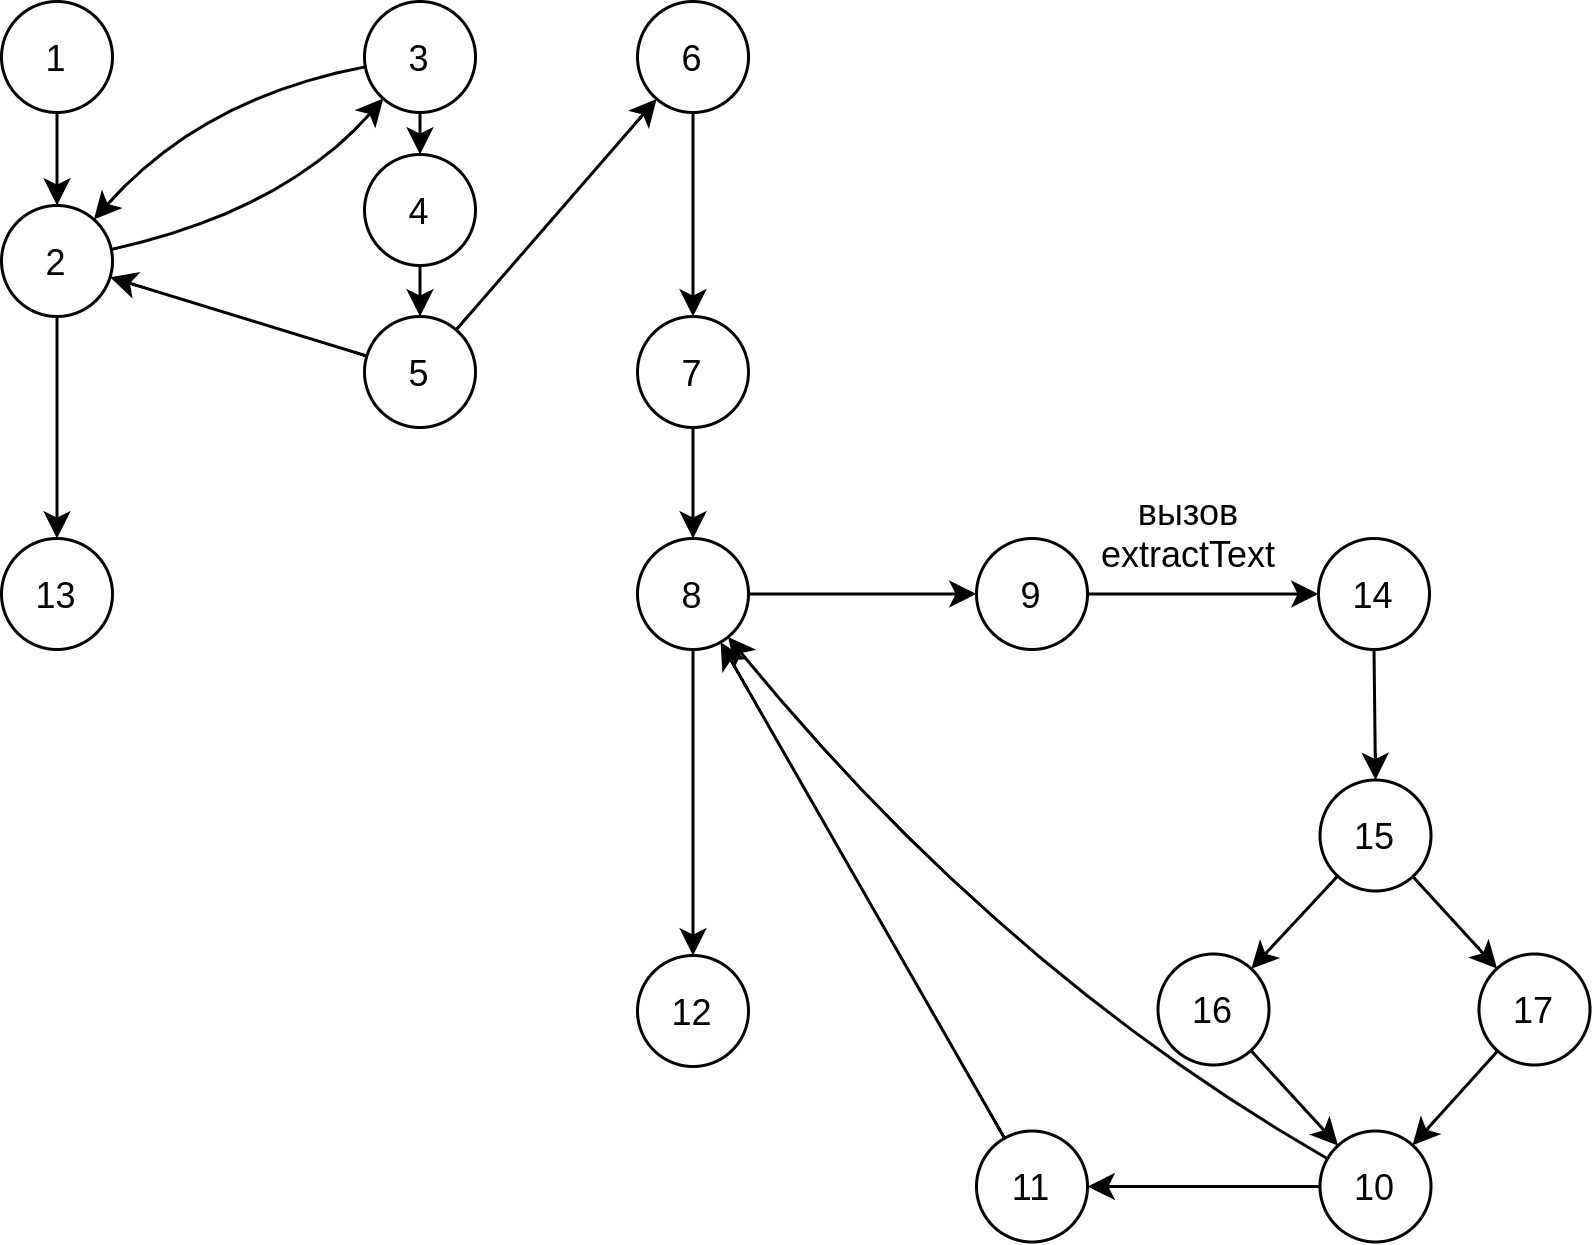
\includegraphics[width=\textwidth]{control.drawio.png}
  \caption{Граф управления для фрагмента кода}
  \label{fig:control}
\end{figure}

\section{Информационный граф}

Информационный граф описывает передачу данных между командами. На нём описываются какие данные передаются от команды к командам.

Информационный граф для фрагмента кода представлен на рисунке~\ref{fig:info}.

\begin{figure}[h!]
  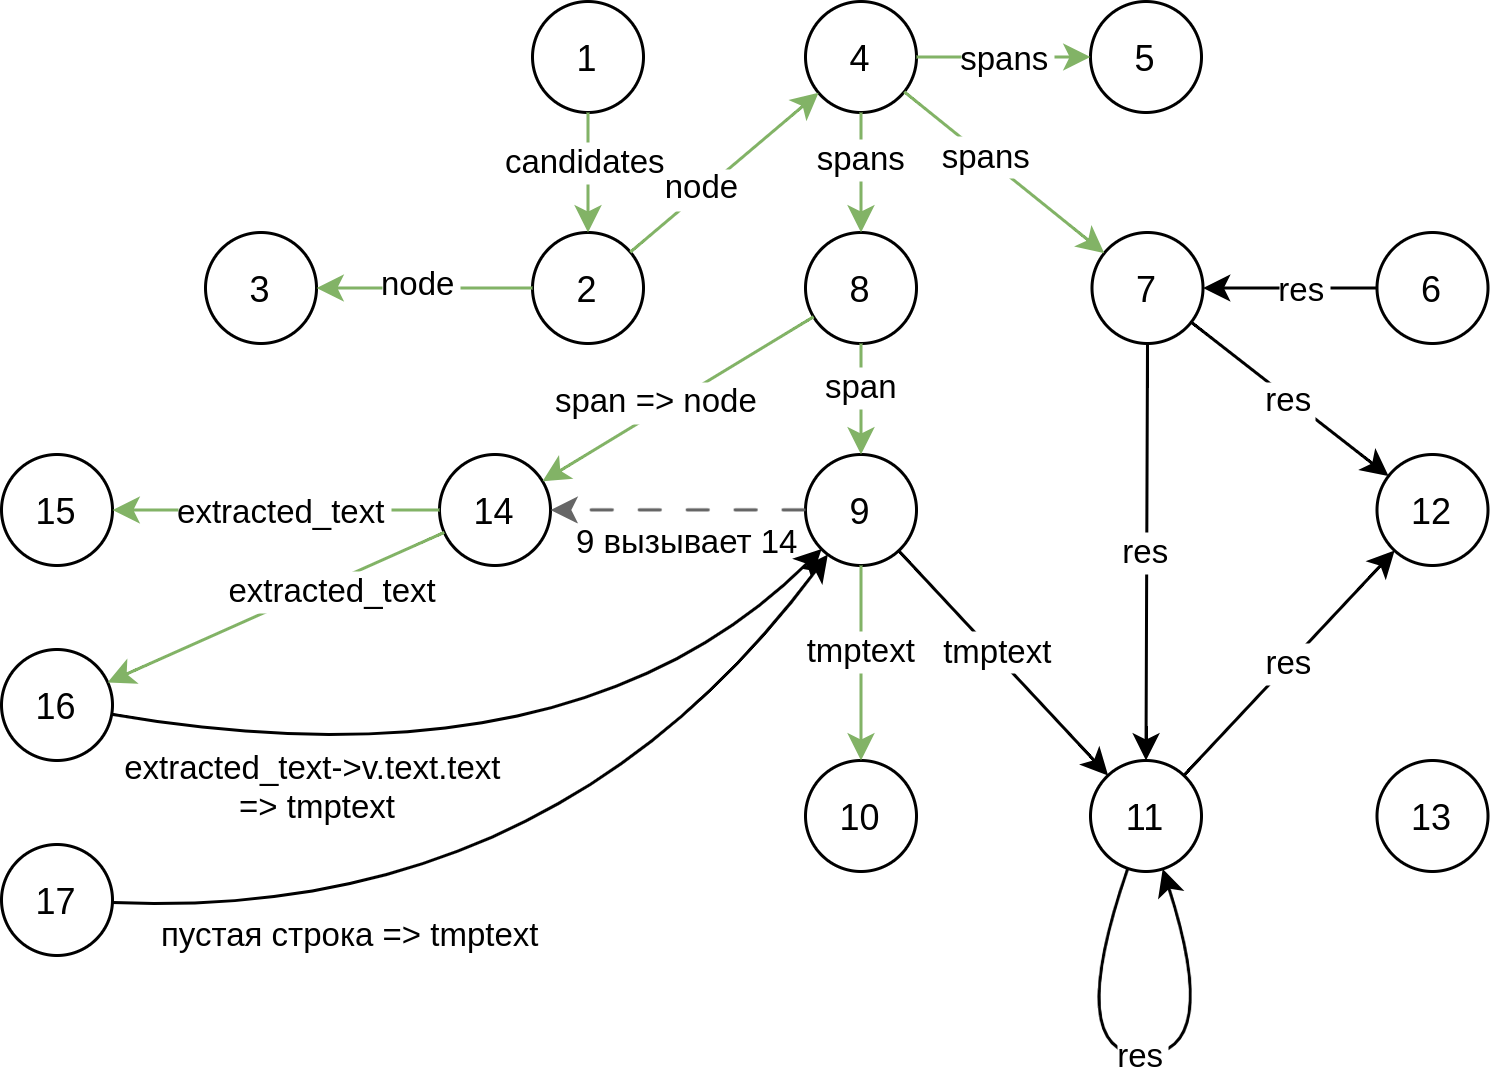
\includegraphics[width=\textwidth]{info.drawio.png}
  \caption{Информационный граф для фрагмента кода}
  \label{fig:info}
\end{figure}

Зелёными стрелками отмечена передача константы. То есть те ситуации, когда переданная информация точно не будет изменена.

Пунктирная стрелка от 9 к 14 означает комментарий. Она не является частью информационного графа.

Знаком ``=>'' отмечено изменение имени переменной при передаче её между функциями.

Это также сделано для упрощения чтения модели.

Дуги из вершин 16 и 17 возвращаются в дугу 9, так как работает оператор = на возвращённое из функции значение.

Вершина 13 означает возврат пустого массива. Ей не нужны никакие данные, так как это возврат константы.

\section{Операционная история}

Операционная история, описывает отношение управления в контексте некоторого определённого запуска программы.

В таком графе каждая вершина имеет не более одного входа и одного выхода.

Операционная история для фрагмента кода представлена на рисунке~\ref{fig:operation}.

\begin{figure}[h!]
  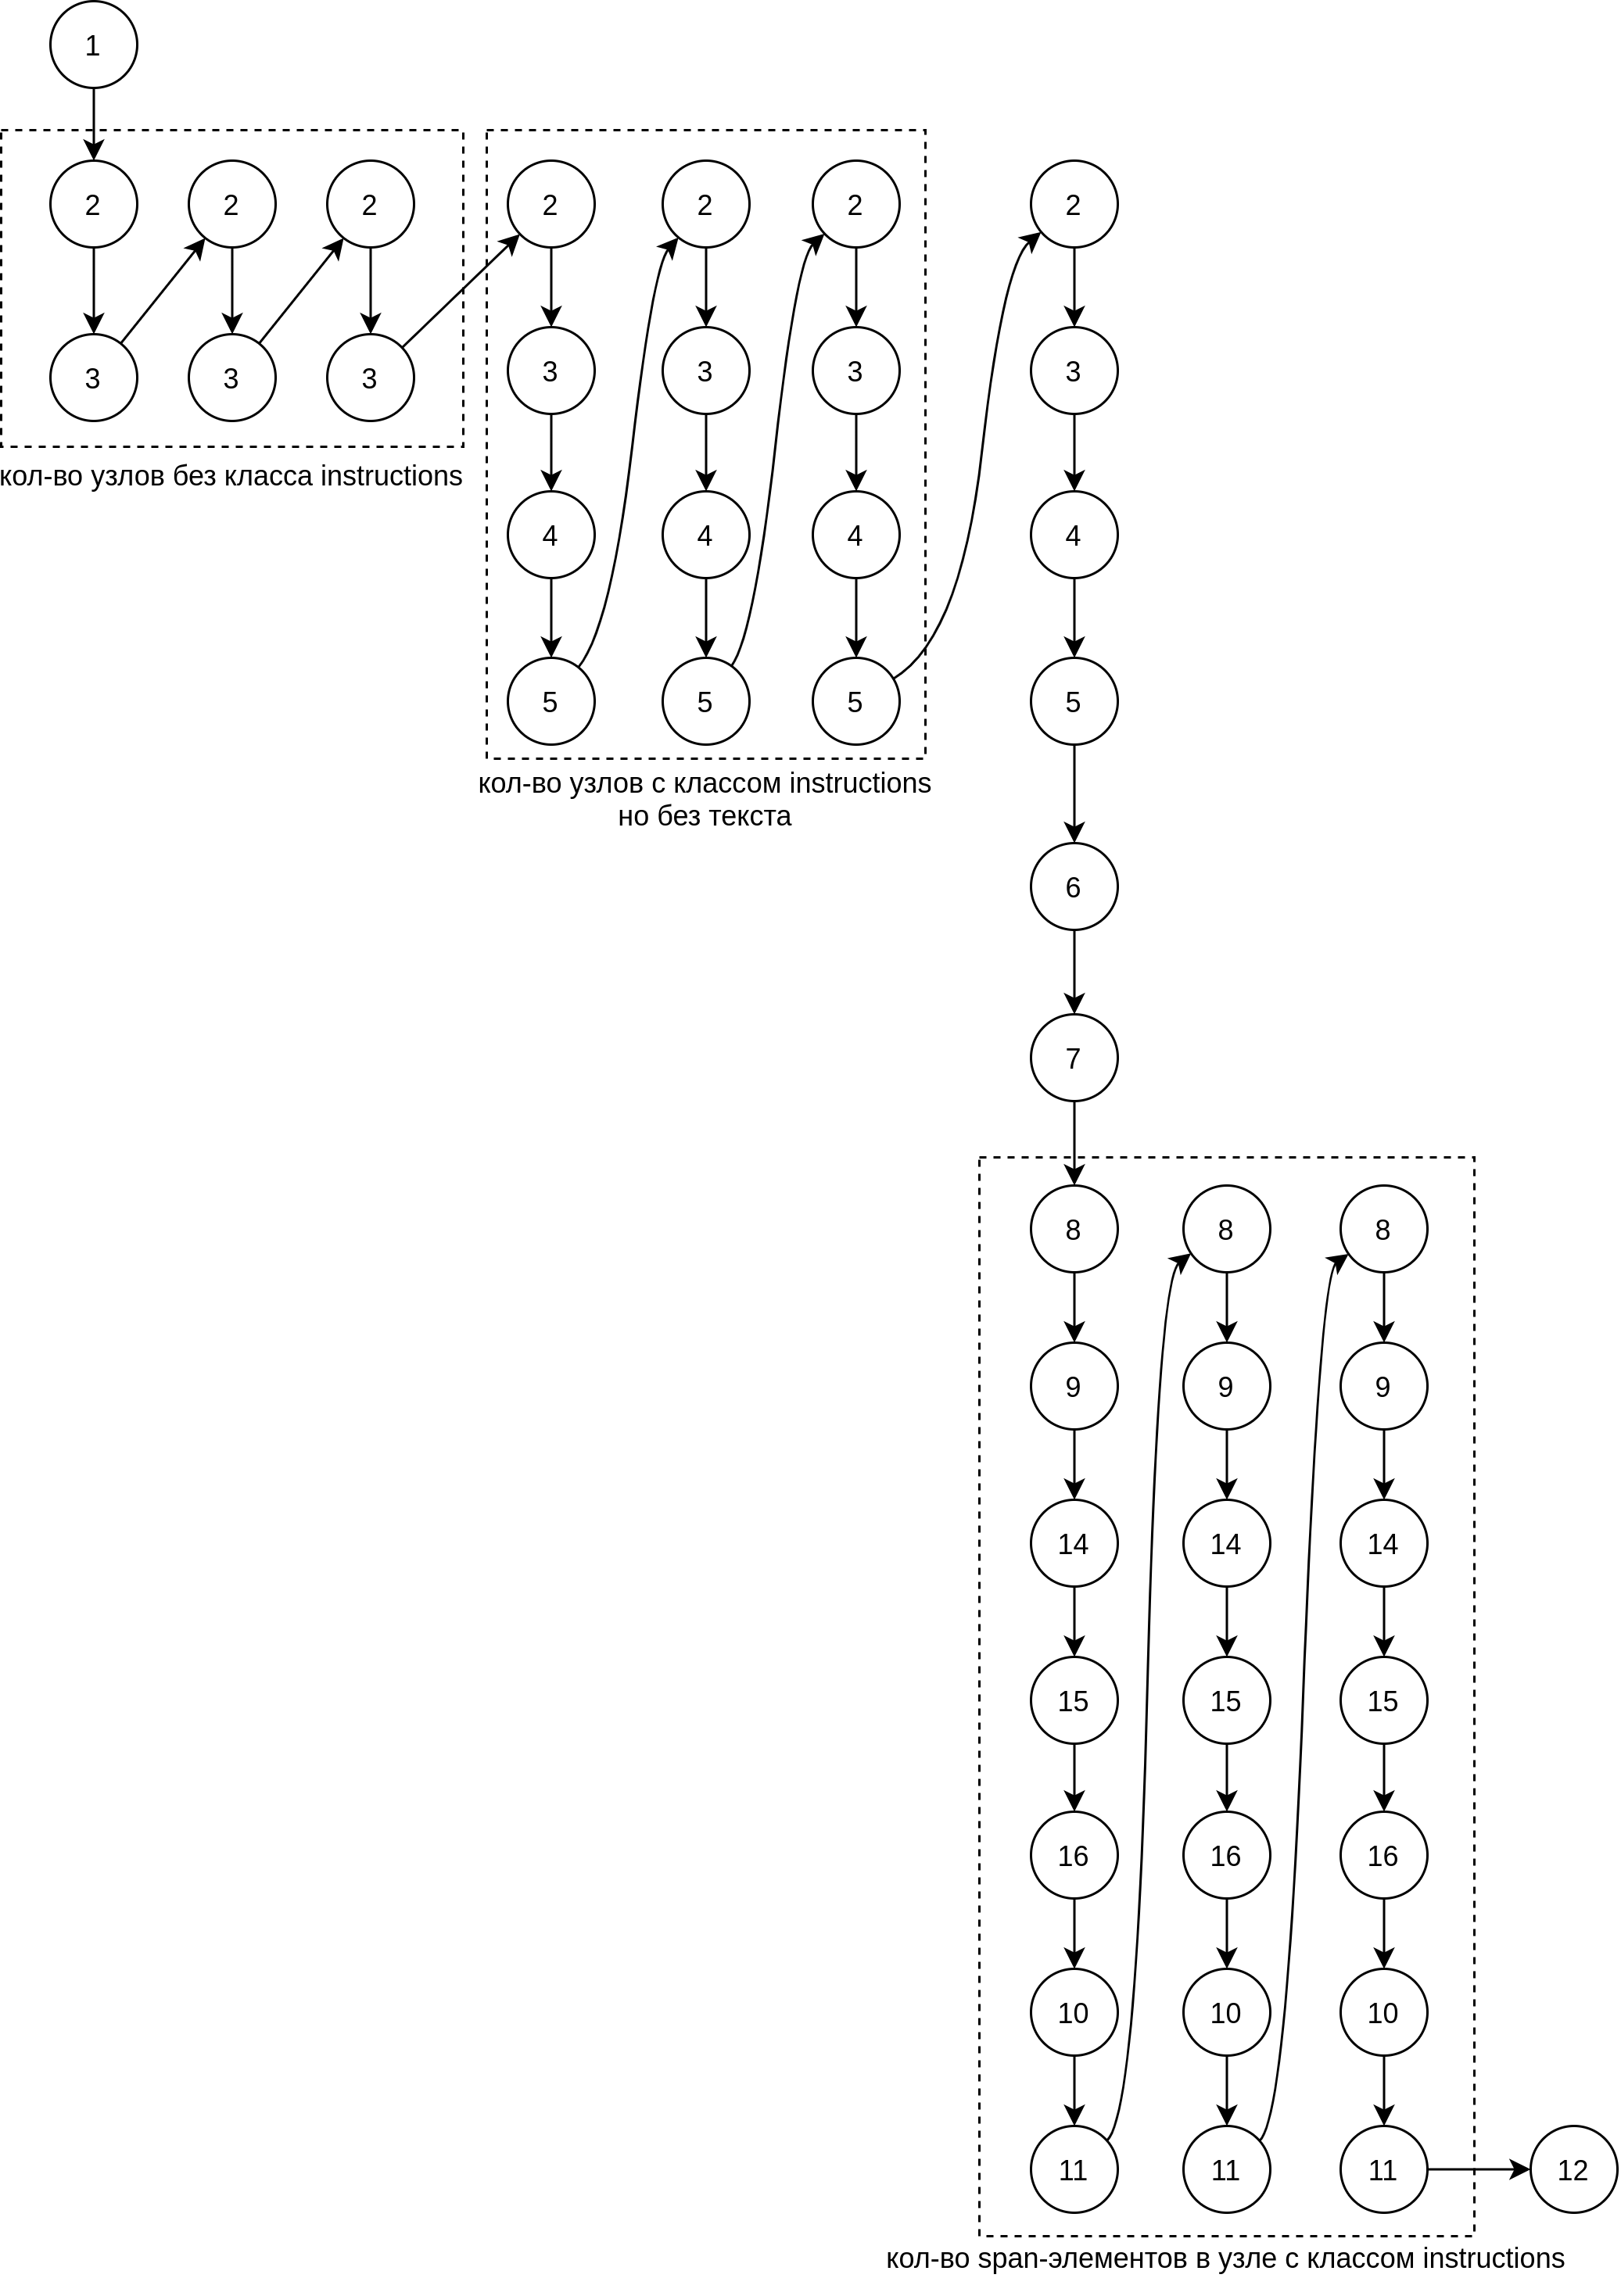
\includegraphics[width=\textwidth]{operation.drawio.png}
  \caption{Операционная история для фрагмента кода}
  \label{fig:operation}
\end{figure}

Оказалось, что в данном фрагменте кода расположен не двойной вложенный цикл, а два цикла: один для фильтрации подходящих элементов и выбора первого из них, а второй --- для обработки его содержимого. Хотя технически в коде один цикл for вложен во второй. 

С одной стороны, выбор фрагмента кода не верен, но с другой --- это один из случаев, в котором использование графовых моделей алгоритма позволило выявить спорное архитектурное решение.

\section{Информационная история}

Информационная история содержит информацию о том, какие команды требовали информацию от других команд в контексте некоторого определённого запуска программы.

Информационная история для фрагмента кода представлена на рисунке~\ref{fig:infohistory}.

\begin{figure}[h!]
  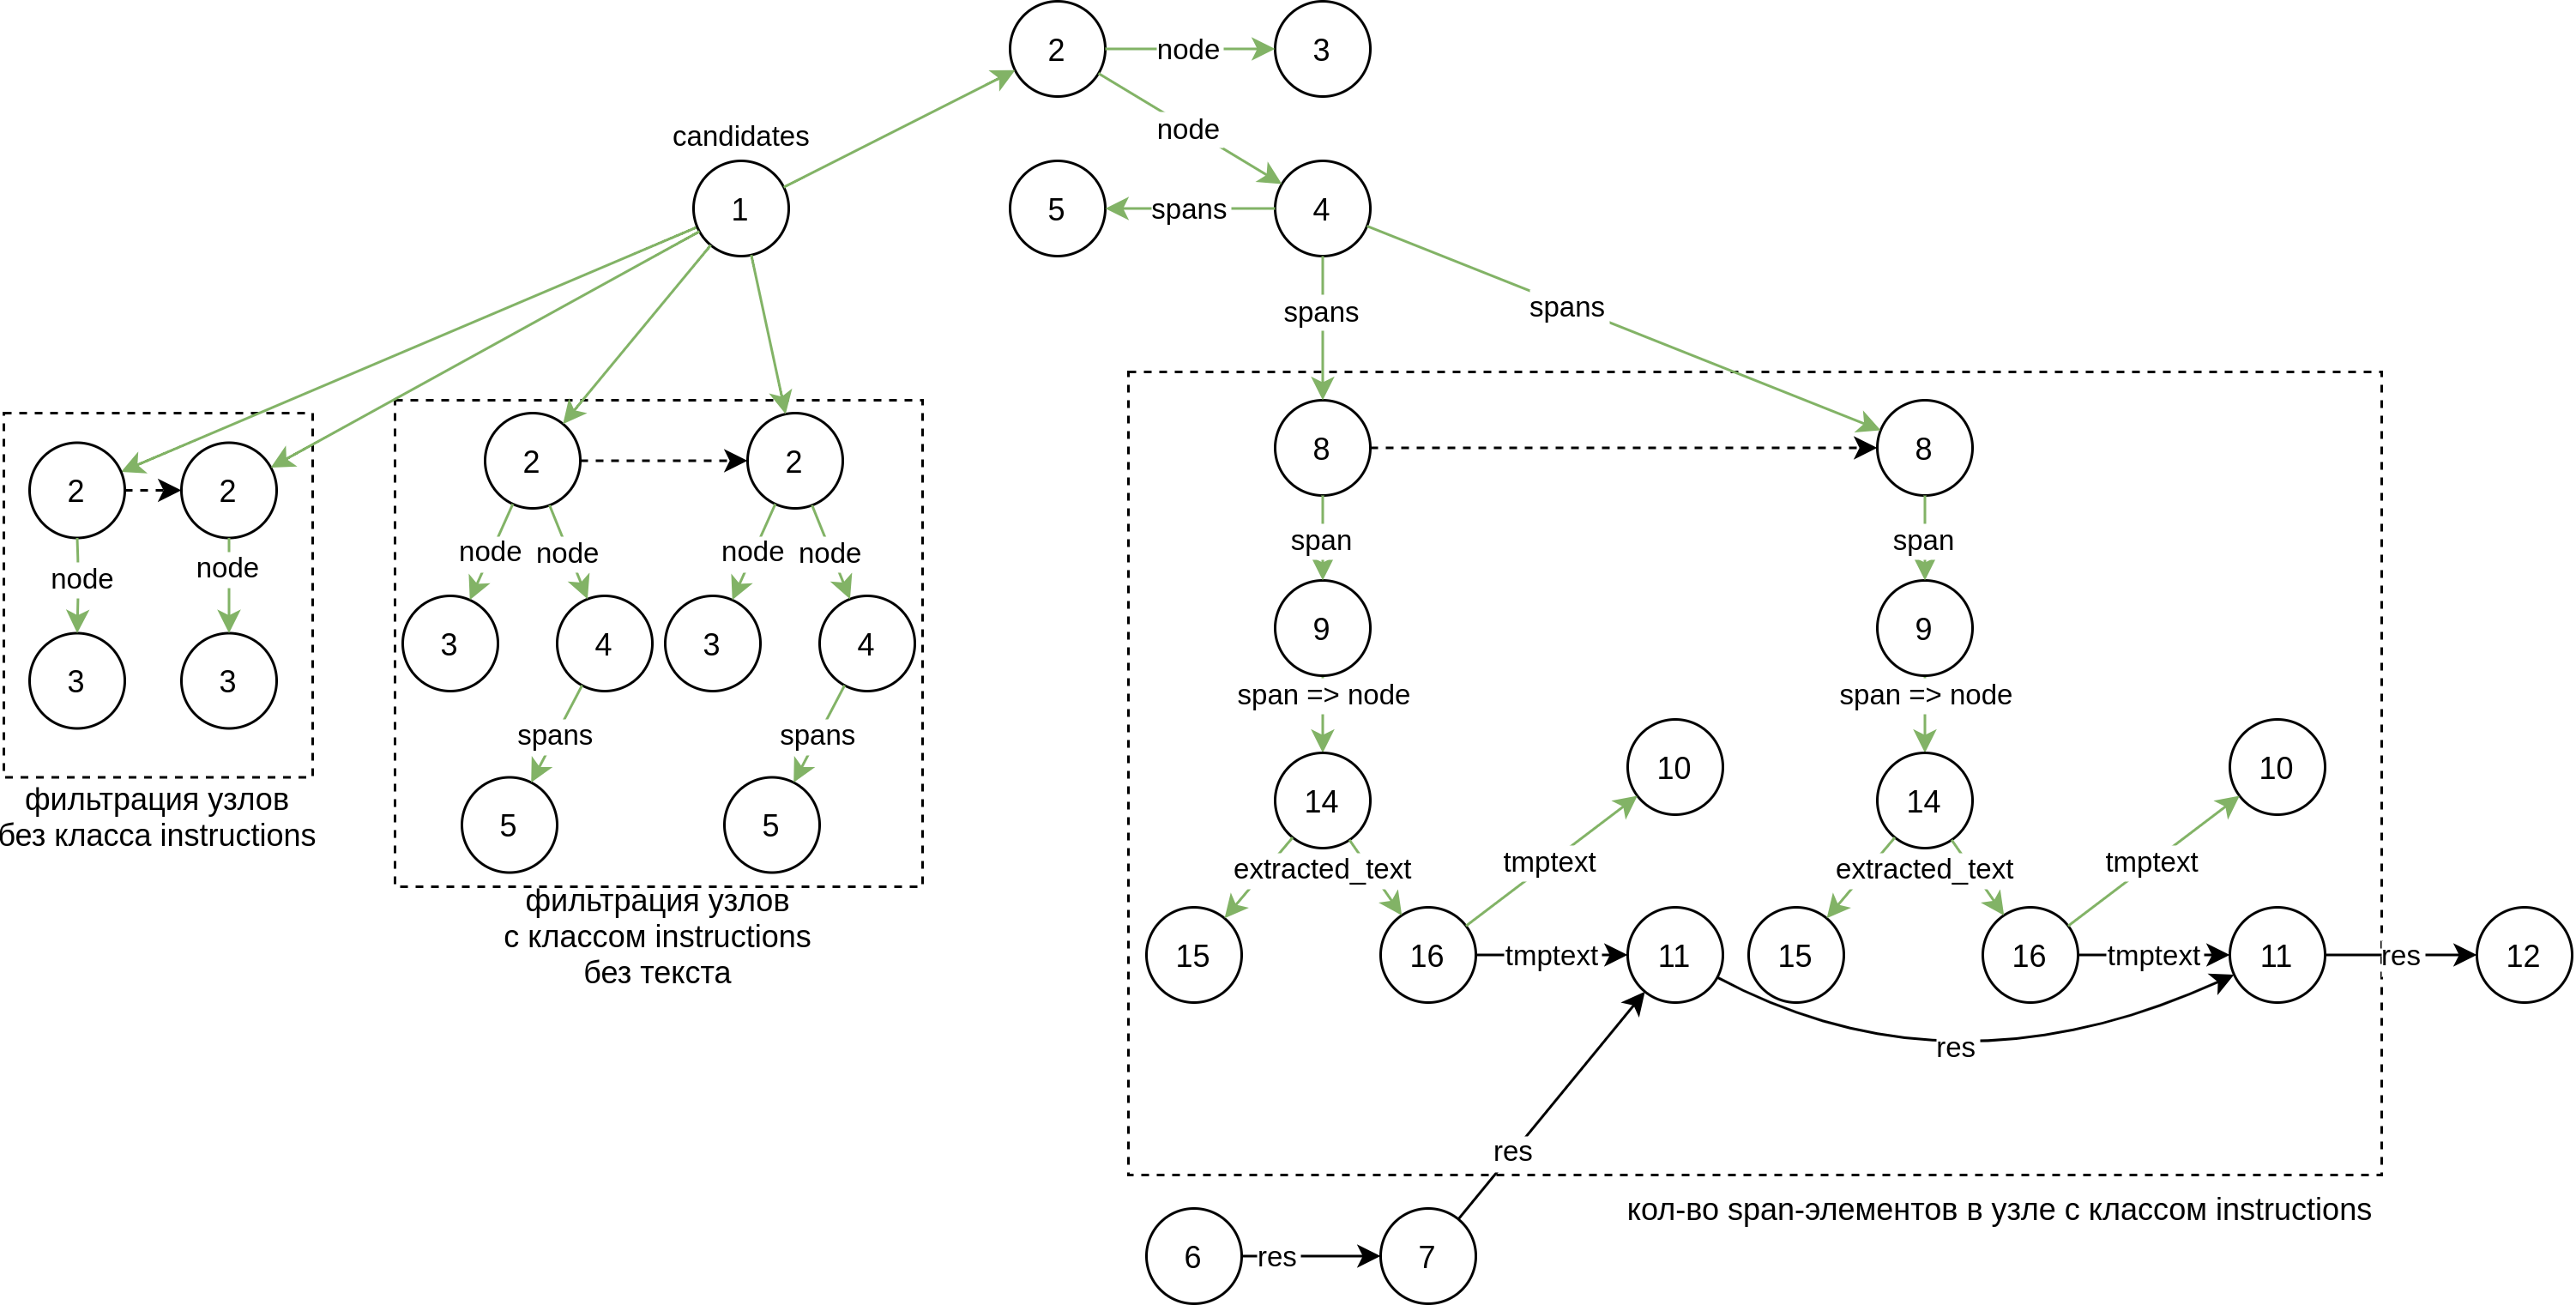
\includegraphics[width=\textwidth]{infohistory.drawio.png}
  \caption{Информационная история для фрагмента кода}
  \label{fig:infohistory}
\end{figure}

На этом рисунке пунктирные квадраты означают комментарии. Пунктирные стрелки --- циклы.

Как в информационном графе, зелёные дуги --- передача константы.